\documentclass[aspectratio=169]{beamer}
\usetheme{Madrid}
\usecolortheme{default}

\usepackage{amsmath}
\usepackage{amssymb}
\usepackage{amsthm}
\usepackage{tikz}
\usepackage{pgfplots}
\pgfplotsset{compat=1.17}

% Remove navigation symbols
\setbeamertemplate{navigation symbols}{}

\title{Trigonometric Functions \& Domain/Range}
\author{Mathematics for ML}
\date{\today}

\begin{document}

\frame{\titlepage}

\begin{frame}{Outline}
\tableofcontents
\end{frame}

\section{Domain and Range}

\begin{frame}{Domain and Range: Definitions}
\begin{definition}[Domain]
The \textbf{domain} of a function $f: A \to B$ is the set of all possible input values $x$ for which $f(x)$ is defined.

$$\text{Domain}(f) = \{x \in A : f(x) \text{ exists}\}$$
\end{definition}

\vspace{0.3cm}

\begin{definition}[Range (Image)]
The \textbf{range} (or \textbf{image}) of a function $f$ is the set of all possible output values.

$$\text{Range}(f) = \{y \in B : \exists x \in \text{Domain}(f) \text{ such that } f(x) = y\}$$
\end{definition}

\vspace{0.3cm}

\textbf{Key Point:} Range $\subseteq$ Codomain, but they may not be equal!
\end{frame}

\begin{frame}{Visual Understanding}
\begin{center}
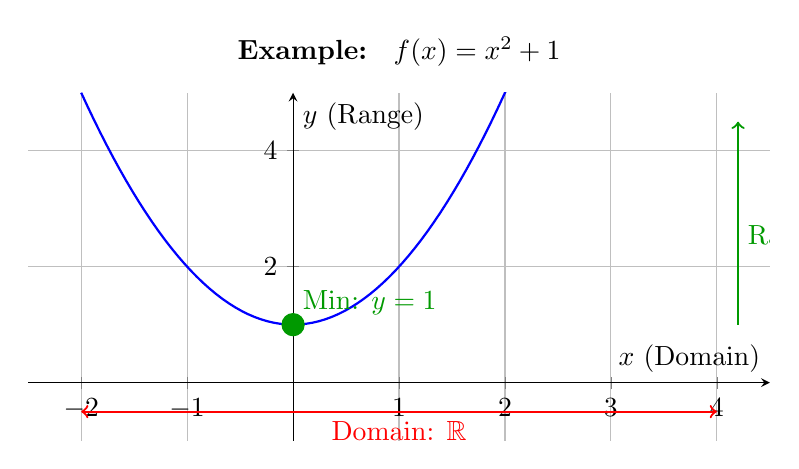
\begin{tikzpicture}
\begin{axis}[
    axis lines=middle,
    xlabel={$x$ (Domain)},
    ylabel={$y$ (Range)},
    domain=-2:4,
    samples=100,
    width=11cm,
    height=6cm,
    ymin=-1, ymax=5,
    xmin=-2.5, xmax=4.5,
    grid=major,
    title={\textbf{Example: } $f(x) = x^2 + 1$}
]
\addplot[blue, thick] {x^2 + 1};

% Show domain
\draw[red, thick, <->] (axis cs:-2, -0.5) -- (axis cs:4, -0.5);
\node[red, below] at (axis cs:1, -0.5) {Domain: $\mathbb{R}$};

% Show range
\draw[green!60!black, thick, ->] (axis cs:4.2, 1) -- (axis cs:4.2, 4.5);
\node[green!60!black, right] at (axis cs:4.2, 2.5) {Range: $[1, \infty)$};

% Mark minimum
\addplot[green!60!black, only marks, mark=*, mark size=4pt] coordinates {(0, 1)};
\node[above right, green!60!black] at (axis cs:0, 1) {Min: $y=1$};
\end{axis}
\end{tikzpicture}
\end{center}
\end{frame}

\begin{frame}{Finding Domain: Common Restrictions}
\textbf{What restricts the domain?}

\vspace{0.3cm}

\begin{enumerate}
    \item \textbf{Division by zero:} $f(x) = \frac{1}{x-2}$ \quad Domain: $x \neq 2$
    
    \item \textbf{Square roots (even roots):} $f(x) = \sqrt{x-3}$ \quad Domain: $x \geq 3$
    
    \item \textbf{Logarithms:} $f(x) = \ln(x)$ \quad Domain: $x > 0$
    
    \item \textbf{Combinations:} $f(x) = \frac{\sqrt{4-x^2}}{x-1}$ \quad Domain: $[-2, 1) \cup (1, 2]$
    \begin{itemize}
        \item Need $4-x^2 \geq 0 \Rightarrow -2 \leq x \leq 2$
        \item Need $x \neq 1$
    \end{itemize}
\end{enumerate}

\vspace{0.3cm}

\textbf{Rule:} Domain is all real numbers \textit{except} where function is undefined.
\end{frame}

\begin{frame}{Finding Range: Strategies}
\textbf{Methods to find range:}

\vspace{0.3cm}

\begin{enumerate}
    \item \textbf{Graphical:} Sketch the function and observe $y$-values
    
    \item \textbf{Algebraic:} Solve $y = f(x)$ for $x$ in terms of $y$
    \begin{itemize}
        \item If $x$ exists for all $y$, then $y$ is in range
        \item Look for restrictions on $y$
    \end{itemize}
    
    \item \textbf{Calculus:} Find critical points, limits at boundaries
    \begin{itemize}
        \item Local extrema give range boundaries
        \item Check behavior as $x \to \pm\infty$
    \end{itemize}
    
    \item \textbf{Known functions:} Use standard ranges
    \begin{itemize}
        \item $x^2$: Range $[0, \infty)$
        \item $e^x$: Range $(0, \infty)$
        \item $\ln(x)$: Range $\mathbb{R}$
    \end{itemize}
\end{enumerate}
\end{frame}

\begin{frame}{Example 1: Finding Domain and Range}
\textbf{Problem:} Find domain and range of $f(x) = \frac{x+1}{x-2}$

\vspace{0.3cm}

\textbf{Solution:}

\textbf{Domain:}
\begin{itemize}
    \item Denominator cannot be zero: $x - 2 \neq 0$
    \item Domain: $\mathbb{R} \setminus \{2\} = (-\infty, 2) \cup (2, \infty)$
\end{itemize}

\vspace{0.3cm}

\textbf{Range:} Solve for $x$ in terms of $y$:
\begin{align*}
y &= \frac{x+1}{x-2} \\
y(x-2) &= x+1 \\
yx - 2y &= x + 1 \\
yx - x &= 1 + 2y \\
x(y-1) &= 1 + 2y \\
x &= \frac{1+2y}{y-1}
\end{align*}

This exists for all $y$ except $y = 1$. Range: $\mathbb{R} \setminus \{1\}$
\end{frame}

\begin{frame}{Example 2: With Square Root}
\textbf{Problem:} Find domain and range of $f(x) = \sqrt{9-x^2}$

\vspace{0.3cm}

\textbf{Solution:}

\textbf{Domain:} Need $9 - x^2 \geq 0$
\begin{align*}
9 - x^2 &\geq 0 \\
9 &\geq x^2 \\
-3 &\leq x \leq 3
\end{align*}
Domain: $[-3, 3]$

\vspace{0.3cm}

\textbf{Range:} 
\begin{itemize}
    \item This is the upper half of a circle with radius 3
    \item Minimum: $f(\pm 3) = 0$
    \item Maximum: $f(0) = \sqrt{9} = 3$
    \item Range: $[0, 3]$
\end{itemize}
\end{frame}

\begin{frame}{Example 2: Visualization}
\begin{center}
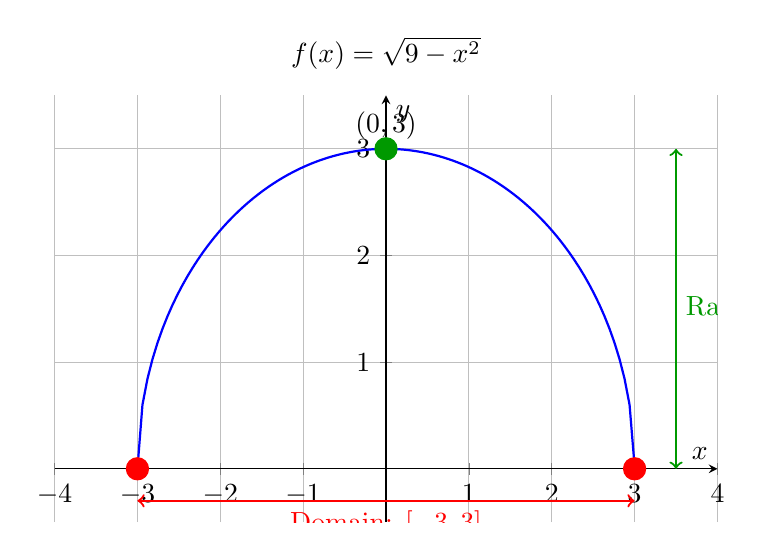
\begin{tikzpicture}
\begin{axis}[
    axis lines=middle,
    xlabel={$x$},
    ylabel={$y$},
    domain=-3:3,
    samples=100,
    width=10cm,
    height=7cm,
    ymin=-0.5, ymax=3.5,
    xmin=-4, xmax=4,
    grid=major,
    title={$f(x) = \sqrt{9-x^2}$}
]
\addplot[blue, thick, domain=-3:3] {sqrt(9-x^2)};

% Mark domain
\draw[red, thick, <->] (axis cs:-3, -0.3) -- (axis cs:3, -0.3);
\node[red, below] at (axis cs:0, -0.3) {Domain: $[-3, 3]$};

% Mark range
\draw[green!60!black, thick, <->] (axis cs:3.5, 0) -- (axis cs:3.5, 3);
\node[green!60!black, right] at (axis cs:3.5, 1.5) {Range: $[0, 3]$};

% Mark key points
\addplot[red, only marks, mark=*, mark size=4pt] coordinates {(-3, 0) (3, 0)};
\addplot[green!60!black, only marks, mark=*, mark size=4pt] coordinates {(0, 3)};
\node[above] at (axis cs:0, 3) {$(0, 3)$};
\end{axis}
\end{tikzpicture}
\end{center}
\end{frame}

\section{Trigonometric Functions}

\begin{frame}{The Unit Circle}
\begin{center}
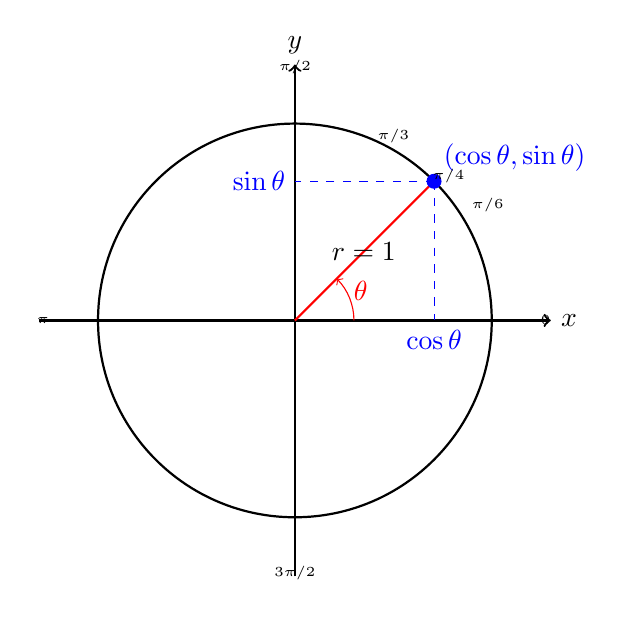
\begin{tikzpicture}[scale=2.5]
% Unit circle
\draw[thick] (0,0) circle (1);

% Axes
\draw[->, thick] (-1.3,0) -- (1.3,0) node[right] {$x$};
\draw[->, thick] (0,-1.3) -- (0,1.3) node[above] {$y$};

% Angle
\draw[red, thick] (0,0) -- (0.707, 0.707);
\draw[red, ->] (0.3,0) arc (0:45:0.3);
\node[red, right] at (0.25, 0.15) {$\theta$};

% Point on circle
\filldraw[blue] (0.707, 0.707) circle (1pt) node[above right] {$(\cos\theta, \sin\theta)$};

% Projections
\draw[dashed, blue] (0.707, 0.707) -- (0.707, 0) node[below] {$\cos\theta$};
\draw[dashed, blue] (0.707, 0.707) -- (0, 0.707) node[left] {$\sin\theta$};

% Special angles marked
\node[right] at (1.2, 0) {\tiny $0$};
\node[above right] at (0.85, 0.5) {\tiny $\pi/6$};
\node[above right] at (0.65, 0.65) {\tiny $\pi/4$};
\node[above] at (0.5, 0.85) {\tiny $\pi/3$};
\node[above] at (0, 1.2) {\tiny $\pi/2$};
\node[left] at (-1.2, 0) {\tiny $\pi$};
\node[below] at (0, -1.2) {\tiny $3\pi/2$};

% Radius = 1
\node at (0.35, 0.35) {$r=1$};
\end{tikzpicture}
\end{center}

\textbf{Definition:} On the unit circle, $\cos\theta$ and $\sin\theta$ are the $x$ and $y$ coordinates.
\end{frame}

\begin{frame}{Basic Trigonometric Functions}
\begin{columns}
\column{0.5\textwidth}
\textbf{Primary Functions:}
\begin{align*}
\sin\theta &= \frac{\text{opposite}}{\text{hypotenuse}} \\[0.3cm]
\cos\theta &= \frac{\text{adjacent}}{\text{hypotenuse}} \\[0.3cm]
\tan\theta &= \frac{\sin\theta}{\cos\theta} = \frac{\text{opposite}}{\text{adjacent}}
\end{align*}

\column{0.5\textwidth}
\textbf{Reciprocal Functions:}
\begin{align*}
\csc\theta &= \frac{1}{\sin\theta} \\[0.3cm]
\sec\theta &= \frac{1}{\cos\theta} \\[0.3cm]
\cot\theta &= \frac{1}{\tan\theta} = \frac{\cos\theta}{\sin\theta}
\end{align*}
\end{columns}

\vspace{0.5cm}

\textbf{Fundamental Identity:}
$$\sin^2\theta + \cos^2\theta = 1$$
\end{frame}

\begin{frame}{Special Angle Values}
\begin{center}
\begin{tabular}{|c|c|c|c|c|c|}
\hline
\textbf{Angle} & $0$ & $\pi/6$ $(30^\circ)$ & $\pi/4$ $(45^\circ)$ & $\pi/3$ $(60^\circ)$ & $\pi/2$ $(90^\circ)$ \\
\hline
\hline
$\sin\theta$ & $0$ & $\frac{1}{2}$ & $\frac{\sqrt{2}}{2}$ & $\frac{\sqrt{3}}{2}$ & $1$ \\
\hline
$\cos\theta$ & $1$ & $\frac{\sqrt{3}}{2}$ & $\frac{\sqrt{2}}{2}$ & $\frac{1}{2}$ & $0$ \\
\hline
$\tan\theta$ & $0$ & $\frac{1}{\sqrt{3}}$ & $1$ & $\sqrt{3}$ & undefined \\
\hline
\end{tabular}
\end{center}

\vspace{0.5cm}

\textbf{Memory Aid:}
$$\sin(0, 30, 45, 60, 90) = \frac{\sqrt{0}}{2}, \frac{\sqrt{1}}{2}, \frac{\sqrt{2}}{2}, \frac{\sqrt{3}}{2}, \frac{\sqrt{4}}{2}$$

$$\cos(0, 30, 45, 60, 90) = \frac{\sqrt{4}}{2}, \frac{\sqrt{3}}{2}, \frac{\sqrt{2}}{2}, \frac{\sqrt{1}}{2}, \frac{\sqrt{0}}{2}$$
\end{frame}

\begin{frame}{Sine Function: $y = \sin(x)$}
\begin{center}
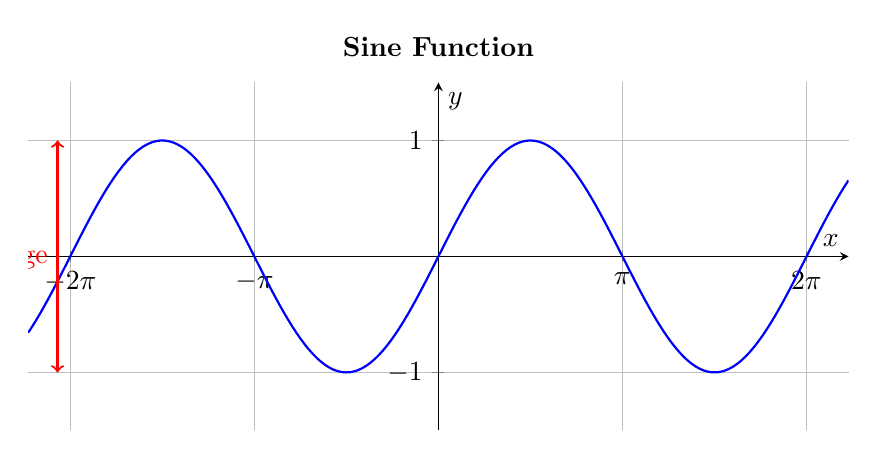
\begin{tikzpicture}
\begin{axis}[
    axis lines=middle,
    xlabel={$x$},
    ylabel={$y$},
    domain=-7:7,
    samples=200,
    width=12cm,
    height=6cm,
    ymin=-1.5, ymax=1.5,
    xmin=-7, xmax=7,
    xtick={-6.28, -3.14, 0, 3.14, 6.28},
    xticklabels={$-2\pi$, $-\pi$, $0$, $\pi$, $2\pi$},
    grid=major,
    title={\textbf{Sine Function}}
]
\addplot[blue, thick] {sin(deg(x))};

% Mark range
\draw[red, thick, <->] (axis cs:-6.5, -1) -- (axis cs:-6.5, 1);
\node[red, left] at (axis cs:-6.5, 0) {Range};
\end{axis}
\end{tikzpicture}
\end{center}

\textbf{Properties:}
\begin{itemize}
    \item Domain: $\mathbb{R}$
    \item Range: $[-1, 1]$
    \item Period: $2\pi$
    \item Odd function: $\sin(-x) = -\sin(x)$
\end{itemize}
\end{frame}

\begin{frame}{Cosine Function: $y = \cos(x)$}
\begin{center}
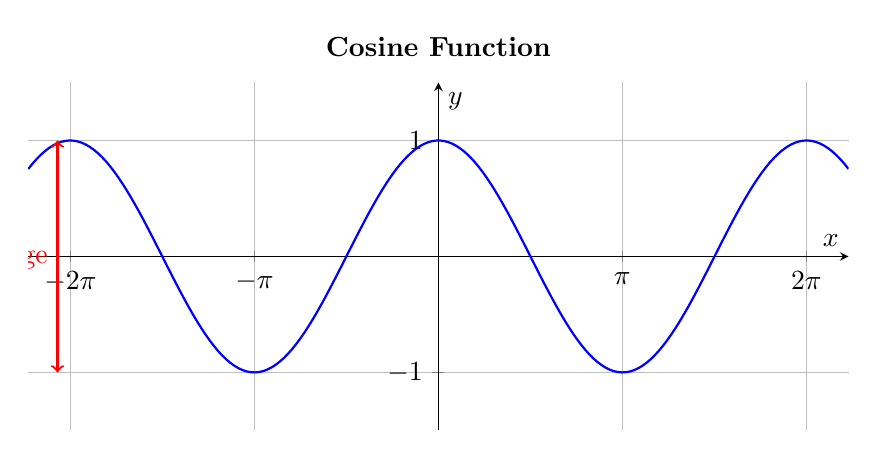
\begin{tikzpicture}
\begin{axis}[
    axis lines=middle,
    xlabel={$x$},
    ylabel={$y$},
    domain=-7:7,
    samples=200,
    width=12cm,
    height=6cm,
    ymin=-1.5, ymax=1.5,
    xmin=-7, xmax=7,
    xtick={-6.28, -3.14, 0, 3.14, 6.28},
    xticklabels={$-2\pi$, $-\pi$, $0$, $\pi$, $2\pi$},
    grid=major,
    title={\textbf{Cosine Function}}
]
\addplot[blue, thick] {cos(deg(x))};

% Mark range
\draw[red, thick, <->] (axis cs:-6.5, -1) -- (axis cs:-6.5, 1);
\node[red, left] at (axis cs:-6.5, 0) {Range};
\end{axis}
\end{tikzpicture}
\end{center}

\textbf{Properties:}
\begin{itemize}
    \item Domain: $\mathbb{R}$
    \item Range: $[-1, 1]$
    \item Period: $2\pi$
    \item Even function: $\cos(-x) = \cos(x)$
\end{itemize}
\end{frame}

\begin{frame}{Tangent Function: $y = \tan(x)$}
\begin{center}
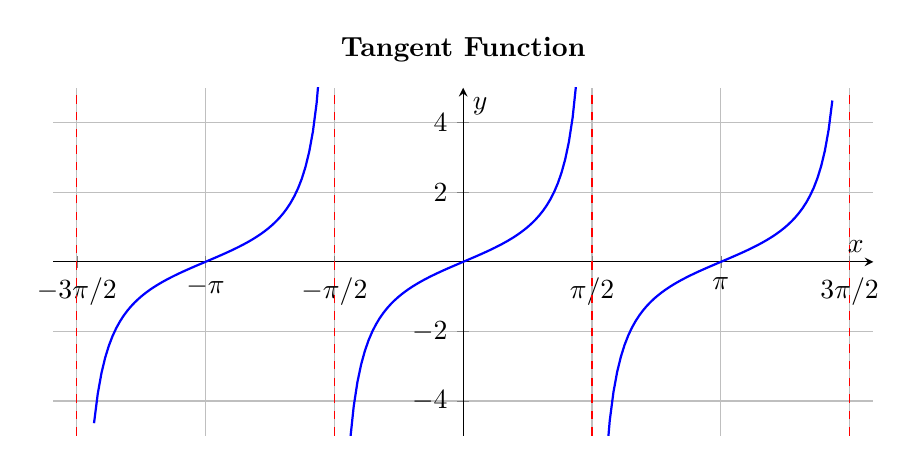
\begin{tikzpicture}
\begin{axis}[
    axis lines=middle,
    xlabel={$x$},
    ylabel={$y$},
    domain=-4.5:4.5,
    samples=200,
    width=12cm,
    height=6cm,
    ymin=-5, ymax=5,
    xmin=-5, xmax=5,
    xtick={-4.71, -3.14, -1.57, 0, 1.57, 3.14, 4.71},
    xticklabels={$-3\pi/2$, $-\pi$, $-\pi/2$, $0$, $\pi/2$, $\pi$, $3\pi/2$},
    grid=major,
    title={\textbf{Tangent Function}},
    restrict y to domain=-10:10
]
\addplot[blue, thick, unbounded coords=jump] {tan(deg(x))};

% Mark asymptotes
\addplot[red, dashed] coordinates {(-1.57, -5) (-1.57, 5)};
\addplot[red, dashed] coordinates {(1.57, -5) (1.57, 5)};
\addplot[red, dashed] coordinates {(4.71, -5) (4.71, 5)};
\addplot[red, dashed] coordinates {(-4.71, -5) (-4.71, 5)};
\end{axis}
\end{tikzpicture}
\end{center}

\textbf{Properties:}
\begin{itemize}
    \item Domain: $\mathbb{R} \setminus \{\frac{\pi}{2} + n\pi : n \in \mathbb{Z}\}$
    \item Range: $\mathbb{R}$
    \item Period: $\pi$
    \item Vertical asymptotes at $x = \frac{\pi}{2} + n\pi$
\end{itemize}
\end{frame}

\begin{frame}{Domain and Range of Trig Functions}
\begin{center}
\small
\begin{tabular}{|l|c|c|c|}
\hline
\textbf{Function} & \textbf{Domain} & \textbf{Range} & \textbf{Period} \\
\hline
\hline
$\sin(x)$ & $\mathbb{R}$ & $[-1, 1]$ & $2\pi$ \\
\hline
$\cos(x)$ & $\mathbb{R}$ & $[-1, 1]$ & $2\pi$ \\
\hline
$\tan(x)$ & $\mathbb{R} \setminus \{\frac{\pi}{2} + n\pi\}$ & $\mathbb{R}$ & $\pi$ \\
\hline
$\csc(x)$ & $\mathbb{R} \setminus \{n\pi\}$ & $(-\infty, -1] \cup [1, \infty)$ & $2\pi$ \\
\hline
$\sec(x)$ & $\mathbb{R} \setminus \{\frac{\pi}{2} + n\pi\}$ & $(-\infty, -1] \cup [1, \infty)$ & $2\pi$ \\
\hline
$\cot(x)$ & $\mathbb{R} \setminus \{n\pi\}$ & $\mathbb{R}$ & $\pi$ \\
\hline
\end{tabular}
\end{center}

\vspace{0.5cm}

\textbf{Key Observations:}
\begin{itemize}
    \item $\sin$ and $\cos$ are bounded: $|\sin x| \leq 1$, $|\cos x| \leq 1$
    \item $\tan$ and $\cot$ are unbounded
    \item $\csc$ and $\sec$ cannot have values in $(-1, 1)$
\end{itemize}
\end{frame}

\begin{frame}{Inverse Trigonometric Functions}
\textbf{To define inverses, restrict domain:}

\vspace{0.3cm}

\begin{center}
\begin{tabular}{|l|c|c|}
\hline
\textbf{Function} & \textbf{Domain} & \textbf{Range} \\
\hline
\hline
$\arcsin(x)$ or $\sin^{-1}(x)$ & $[-1, 1]$ & $[-\pi/2, \pi/2]$ \\
\hline
$\arccos(x)$ or $\cos^{-1}(x)$ & $[-1, 1]$ & $[0, \pi]$ \\
\hline
$\arctan(x)$ or $\tan^{-1}(x)$ & $\mathbb{R}$ & $(-\pi/2, \pi/2)$ \\
\hline
\end{tabular}
\end{center}

\vspace{0.5cm}

\textbf{Properties:}
\begin{itemize}
    \item $\sin(\arcsin(x)) = x$ for $x \in [-1, 1]$
    \item $\arcsin(\sin(x)) = x$ for $x \in [-\pi/2, \pi/2]$
    \item Similar identities hold for $\arccos$ and $\arctan$
\end{itemize}

\vspace{0.3cm}

\textbf{Note:} Domain of inverse = Range of original (restricted)
\end{frame}

\begin{frame}{Arctangent Function: $y = \arctan(x)$}
\begin{center}
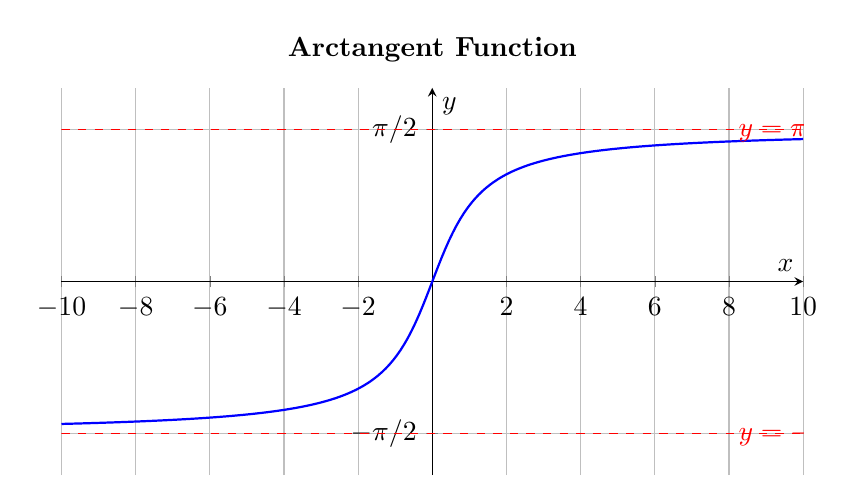
\begin{tikzpicture}
\begin{axis}[
    axis lines=middle,
    xlabel={$x$},
    ylabel={$y$},
    domain=-10:10,
    samples=200,
    width=11cm,
    height=6.5cm,
    ymin=-2, ymax=2,
    xmin=-10, xmax=10,
    ytick={-1.57, 0, 1.57},
    yticklabels={$-\pi/2$, $0$, $\pi/2$},
    grid=major,
    title={\textbf{Arctangent Function}}
]
\addplot[blue, thick] {atan(x)*pi/180};

% Horizontal asymptotes
\addplot[red, dashed] coordinates {(-10, 1.57) (10, 1.57)};
\addplot[red, dashed] coordinates {(-10, -1.57) (10, -1.57)};
\node[red, right] at (axis cs:8, 1.57) {$y = \pi/2$};
\node[red, right] at (axis cs:8, -1.57) {$y = -\pi/2$};
\end{axis}
\end{tikzpicture}
\end{center}

Domain: $\mathbb{R}$, \quad Range: $(-\pi/2, \pi/2)$

Horizontal asymptotes at $y = \pm\pi/2$
\end{frame}

\begin{frame}{Trigonometric Identities}
\textbf{Pythagorean Identities:}
\begin{align*}
\sin^2\theta + \cos^2\theta &= 1 \\
1 + \tan^2\theta &= \sec^2\theta \\
1 + \cot^2\theta &= \csc^2\theta
\end{align*}

\vspace{0.3cm}

\textbf{Angle Addition:}
\begin{align*}
\sin(\alpha \pm \beta) &= \sin\alpha\cos\beta \pm \cos\alpha\sin\beta \\
\cos(\alpha \pm \beta) &= \cos\alpha\cos\beta \mp \sin\alpha\sin\beta
\end{align*}

\vspace{0.3cm}

\textbf{Double Angle:}
\begin{align*}
\sin(2\theta) &= 2\sin\theta\cos\theta \\
\cos(2\theta) &= \cos^2\theta - \sin^2\theta = 1 - 2\sin^2\theta = 2\cos^2\theta - 1
\end{align*}
\end{frame}

\begin{frame}{Example 3: Domain of Composite Function}
\textbf{Problem:} Find the domain of $f(x) = \arcsin\left(\frac{x-1}{2}\right)$

\vspace{0.3cm}

\textbf{Solution:}

For $\arcsin(u)$ to be defined, we need $u \in [-1, 1]$.

Here $u = \frac{x-1}{2}$, so:
\begin{align*}
-1 &\leq \frac{x-1}{2} \leq 1 \\
-2 &\leq x-1 \leq 2 \\
-1 &\leq x \leq 3
\end{align*}

\textbf{Domain:} $[-1, 3]$

\vspace{0.3cm}

\textbf{Range:} Since $\frac{x-1}{2}$ covers all values in $[-1, 1]$ as $x$ varies over $[-1, 3]$, and $\arcsin$ has range $[-\pi/2, \pi/2]$:

\textbf{Range:} $[-\pi/2, \pi/2]$
\end{frame}

\begin{frame}{Example 4: Solving Trig Equations}
\textbf{Problem:} Solve $2\sin^2(x) - \sin(x) - 1 = 0$ for $x \in [0, 2\pi]$

\vspace{0.3cm}

\textbf{Solution:}

This is a quadratic in $\sin(x)$. Let $u = \sin(x)$:
\begin{align*}
2u^2 - u - 1 &= 0 \\
(2u + 1)(u - 1) &= 0
\end{align*}

So $u = -\frac{1}{2}$ or $u = 1$.

\vspace{0.3cm}

\textbf{Case 1:} $\sin(x) = 1$ \quad $\Rightarrow$ \quad $x = \frac{\pi}{2}$

\textbf{Case 2:} $\sin(x) = -\frac{1}{2}$ \quad $\Rightarrow$ \quad $x = \frac{7\pi}{6}, \frac{11\pi}{6}$

\vspace{0.3cm}

\textbf{Solutions:} $x \in \left\{\frac{\pi}{2}, \frac{7\pi}{6}, \frac{11\pi}{6}\right\}$
\end{frame}

\begin{frame}{Transformations of Trig Functions}
\textbf{General Form:} $y = A\sin(B(x - C)) + D$ or $y = A\cos(B(x - C)) + D$

\vspace{0.3cm}

\textbf{Parameters:}
\begin{itemize}
    \item $A$: \textbf{Amplitude} (vertical stretch/compression)
    \begin{itemize}
        \item Range becomes $[D-|A|, D+|A|]$
    \end{itemize}
    
    \item $B$: Affects \textbf{period}
    \begin{itemize}
        \item New period: $\frac{2\pi}{|B|}$
    \end{itemize}
    
    \item $C$: \textbf{Phase shift} (horizontal shift)
    \begin{itemize}
        \item Shifts graph $C$ units to the right
    \end{itemize}
    
    \item $D$: \textbf{Vertical shift}
    \begin{itemize}
        \item Shifts graph $D$ units up
    \end{itemize}
\end{itemize}

\vspace{0.3cm}

\textbf{Example:} $y = 3\sin(2x - \pi) + 1$ has amplitude 3, period $\pi$, phase shift $\pi/2$, vertical shift 1.
\end{frame}

\begin{frame}{Example 5: Transformed Function}
\begin{center}
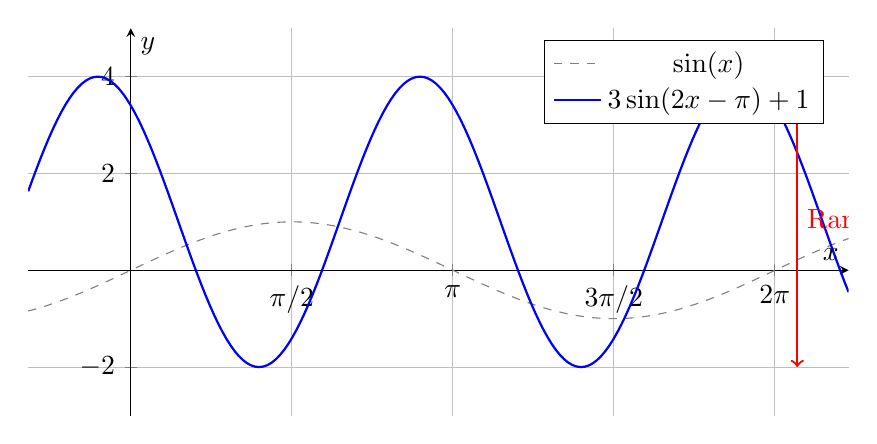
\begin{tikzpicture}
\begin{axis}[
    axis lines=middle,
    xlabel={$x$},
    ylabel={$y$},
    domain=-1:7,
    samples=200,
    width=12cm,
    height=6.5cm,
    ymin=-3, ymax=5,
    xmin=-1, xmax=7,
    xtick={0, 1.57, 3.14, 4.71, 6.28},
    xticklabels={$0$, $\pi/2$, $\pi$, $3\pi/2$, $2\pi$},
    grid=major,
    legend pos=north east
]
% Original
\addplot[gray, dashed] {sin(deg(x))};
\addlegendentry{$\sin(x)$}

% Transformed
\addplot[blue, thick] {3*sin(deg(2*x - 180)) + 1};
\addlegendentry{$3\sin(2x - \pi) + 1$}

% Mark range
\draw[red, thick, <->] (axis cs:6.5, -2) -- (axis cs:6.5, 4);
\node[red, right] at (axis cs:6.5, 1) {Range: $[-2, 4]$};
\end{axis}
\end{tikzpicture}
\end{center}

$y = 3\sin(2x - \pi) + 1$: Amplitude 3, Period $\pi$, Shift right $\pi/2$, Up 1
\end{frame}

\begin{frame}{Applications in Calculus}
\textbf{Derivatives:}
\begin{align*}
\frac{d}{dx}\sin(x) &= \cos(x) \\
\frac{d}{dx}\cos(x) &= -\sin(x) \\
\frac{d}{dx}\tan(x) &= \sec^2(x) \\
\frac{d}{dx}\arcsin(x) &= \frac{1}{\sqrt{1-x^2}} \\
\frac{d}{dx}\arctan(x) &= \frac{1}{1+x^2}
\end{align*}

\vspace{0.3cm}

\textbf{Note:} Domains of derivatives match domains of original functions!
\end{frame}

\begin{frame}{Applications in Optimization}
\textbf{Example:} Maximize area of rectangle inscribed in semicircle of radius $r$.

\begin{center}
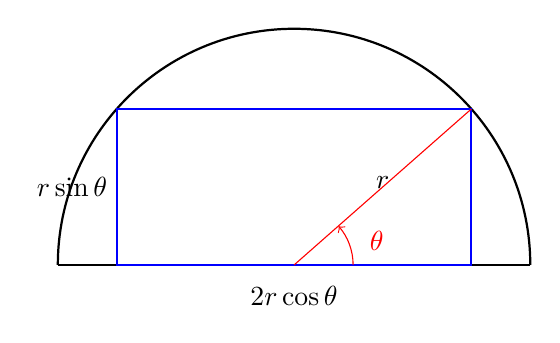
\begin{tikzpicture}[scale=1.5]
% Semicircle
\draw[thick] (-2,0) arc (180:0:2);
\draw[thick] (-2,0) -- (2,0);

% Rectangle
\draw[blue, thick] (-1.5, 0) rectangle (1.5, 1.32);

% Angle and radius
\draw[red] (0,0) -- (1.5, 1.32);
\draw[red, ->] (0.5,0) arc (0:41:0.5);
\node[red] at (0.7, 0.2) {$\theta$};
\node at (0.75, 0.7) {$r$};

% Labels
\node[below] at (0, -0.1) {$2r\cos\theta$};
\node[left] at (-1.5, 0.66) {$r\sin\theta$};
\end{tikzpicture}
\end{center}

\textbf{Solution:} $A(\theta) = 2r\cos\theta \cdot r\sin\theta = r^2\sin(2\theta)$

Domain: $\theta \in [0, \pi/2]$, \quad Maximum at $\theta = \pi/4$, giving $A_{\max} = r^2$
\end{frame}

\section{Summary}

\begin{frame}{Summary: Domain and Range}
\textbf{Key Takeaways:}

\begin{itemize}
    \item \textbf{Domain:} All possible inputs where function is defined
    \begin{itemize}
        \item Check: division by zero, square roots, logarithms
    \end{itemize}
    
    \item \textbf{Range:} All possible outputs
    \begin{itemize}
        \item Methods: graphing, algebra, calculus
    \end{itemize}
    
    \item \textbf{Inverse functions:} Domain and range swap
    
    \item \textbf{Compositions:} Inner function's range must fit outer function's domain
\end{itemize}

\vspace{0.3cm}

\textbf{Remember:} Always verify both domain AND range when working with functions!
\end{frame}

\begin{frame}{Summary: Trigonometric Functions}
\textbf{Essential Knowledge:}

\begin{enumerate}
    \item \textbf{Unit Circle:} $(\cos\theta, \sin\theta)$ for angle $\theta$
    
    \item \textbf{Six Functions:} $\sin, \cos, \tan, \csc, \sec, \cot$
    
    \item \textbf{Domains \& Ranges:}
    \begin{itemize}
        \item $\sin, \cos$: Domain $\mathbb{R}$, Range $[-1, 1]$
        \item $\tan, \cot$: Domain has gaps, Range $\mathbb{R}$
    \end{itemize}
    
    \item \textbf{Identities:} $\sin^2 + \cos^2 = 1$, angle addition, double angle
    
    \item \textbf{Inverse Functions:} Restricted domains to be one-to-one
    
    \item \textbf{Transformations:} Amplitude, period, phase shift, vertical shift
\end{enumerate}
\end{frame}

\begin{frame}{Practice Problems}
\textbf{Domain and Range:}
\begin{enumerate}
    \item Find domain and range of $f(x) = \sqrt{x^2 - 4}$
    \item Find domain of $g(x) = \ln(3-x) + \frac{1}{\sqrt{x-1}}$
    \item Find range of $h(x) = \frac{2x+1}{x+3}$
\end{enumerate}

\vspace{0.3cm}

\textbf{Trigonometry:}
\begin{enumerate}
    \item Solve $\cos(2x) = \frac{1}{2}$ for $x \in [0, 2\pi]$
    \item Find amplitude, period, and phase shift of $y = -2\cos(3x + \pi) - 1$
    \item Simplify $\sin(\arccos(x))$ for $x \in [-1, 1]$
    \item Find domain and range of $f(x) = 2\arctan(x-1) + \pi$
\end{enumerate}
\end{frame}

\begin{frame}{}
\begin{center}
\Huge Thank You!

\vspace{1cm}

\Large Questions?

\vspace{1cm}

\normalsize
\textit{Master these fundamentals — they appear everywhere} \\
\textit{in calculus, optimization, and machine learning!}
\end{center}
\end{frame}

\end{document}
